\documentclass[sigconf,nonacm]{acmart}

\settopmatter{printacmref=false}
\renewcommand\footnotetextcopyrightpermission[1]{}

\usepackage{booktabs}
\usepackage{array}
\usepackage{adjustbox}
\usepackage{graphicx}
\usepackage{subcaption}
\usepackage{tikz}
\usepackage{pgfplots}
\usepackage{listings}
\usepackage{xcolor}
\usepackage{xspace}
\usepackage{amsmath}
\usepackage{placeins}
\usepackage{enumitem}
\usepackage[ruled,vlined,linesnumbered]{algorithm2e}

\usetikzlibrary{arrows.meta,positioning,shapes.geometric}
\pgfplotsset{compat=1.18}

\setlength{\textfloatsep}{7pt plus 2pt minus 2pt}
\setlength{\floatsep}{6pt plus 2pt minus 2pt}
\setlength{\intextsep}{6pt plus 2pt minus 2pt}
\setlist[itemize]{leftmargin=*,topsep=2pt,itemsep=2pt}
\setlist[description]{leftmargin=1.2cm,labelwidth=1.0cm,topsep=2pt,itemsep=2pt}

\definecolor{reluiNavy}{RGB}{22,36,58}
\definecolor{reluiTeal}{RGB}{15,118,110}
\definecolor{reluiCyan}{RGB}{3,105,161}
\definecolor{reluiAmber}{RGB}{181,71,8}
\definecolor{reluiRed}{RGB}{180,35,24}
\definecolor{reluiGreen}{RGB}{2,122,72}
\definecolor{reluiLine}{RGB}{216,224,234}
\definecolor{codeBg}{RGB}{248,250,252}
\definecolor{codeKeyword}{RGB}{88,28,135}
\definecolor{codeString}{RGB}{3,105,161}
\definecolor{codeComment}{RGB}{71,85,105}

\lstdefinestyle{reluiCode}{
  backgroundcolor=\color{codeBg},
  basicstyle=\ttfamily\scriptsize,
  breaklines=true,
  columns=fullflexible,
  frame=single,
  rulecolor=\color{reluiLine},
  keywordstyle=\color{codeKeyword}\bfseries,
  stringstyle=\color{codeString},
  commentstyle=\color{codeComment},
  showstringspaces=false,
  numbers=left,
  numberstyle=\tiny\color{codeComment},
  numbersep=6pt,
  tabsize=2
}
\lstset{style=reluiCode}

\SetKwInput{KwInput}{Input}
\SetKwInput{KwOutput}{Output}

\newcommand{\RelUI}{RelUI\xspace}
\newcommand{\yes}{Yes}
\newcommand{\no}{--}
\newcommand{\artifacttable}[1]{%
  \IfFileExists{../artifacts/tables/#1.tex}{\input{../artifacts/tables/#1.tex}}{\input{artifacts/tables/#1.tex}}%
}
\newcommand{\artifactimage}[2][]{%
  \IfFileExists{../#2}{\includegraphics[#1]{../#2}}{\includegraphics[#1]{#2}}%
}

\begin{document}

\title{RelUI: Relational Behavioral Consistency Testing for Web UIs}
\subtitle{CS 527 Research Project Report: Group 2}

\author{Ajmal Ali}
\author{Muneeb Hoda}
\affiliation{%
  \institution{University of Illinois at Urbana-Champaign}
  \city{Urbana}
  \state{Illinois}
  \country{USA}
}
\email{{aali274,shoda6}@illinois.edu}

\begin{abstract}
Modern Web UI bugs often hide between pages rather than inside one page. A confirmation screen can look normal while losing data after back navigation; a protected dashboard can render correctly while being reachable without login. This paper presents \RelUI, a TypeScript and Playwright prototype for relational behavioral consistency testing of Web UIs. \RelUI explores browser traces, canonicalizes states, infers a state-transition graph, and checks explicit workflow invariants over traces and endpoints. We evaluate the final artifact on four benchmark workflows, 20 subject variants, and 16 injected faults. The final run explored 454 replayable traces, discovered 230 canonical states and 467 transitions, detected all 16 injected faults, and reported zero clean false positives in 250.08 seconds. Lightweight structural and visual baselines detected only 5 and 0 faults, respectively, showing that workflow correctness needs relational oracles beyond local DOM or screenshot checks.
\end{abstract}

\maketitle

\section{Introduction}
Web applications increasingly encode critical behavior as multi-step workflows: login, checkout, account settings, and money transfer flows all depend on action history. These workflows fail in ways that are hard to detect with one-state checks. A page can contain the right controls and still violate an authentication precondition; two valid paths can reach the same confirmation URL but disagree about preserved user data.

\RelUI targets this class of bug. It treats a Web UI as an explored transition system and checks relational invariants over traces, graph edges, and endpoint states. The final artifact is implemented in TypeScript on top of Playwright \citep{playwright}; it emits JSON, CSV, HTML, screenshots, and LaTeX-ready tables.

\begin{figure}[t]
  \centering
  \scriptsize
  \setlength{\tabcolsep}{3pt}
  \begin{tabular}{>{\centering\arraybackslash}p{0.22\columnwidth}>{\centering\arraybackslash}p{0.22\columnwidth}>{\centering\arraybackslash}p{0.22\columnwidth}>{\centering\arraybackslash}p{0.22\columnwidth}}
    \fcolorbox{reluiTeal}{reluiTeal!8}{\parbox[c][0.45in][c]{0.19\columnwidth}{\centering\textbf{4}\\apps}} &
    \fcolorbox{reluiCyan}{reluiCyan!8}{\parbox[c][0.45in][c]{0.19\columnwidth}{\centering\textbf{20}\\variants}} &
    \fcolorbox{reluiAmber}{reluiAmber!8}{\parbox[c][0.45in][c]{0.19\columnwidth}{\centering\textbf{16/16}\\faults}} &
    \fcolorbox{reluiGreen}{reluiGreen!8}{\parbox[c][0.45in][c]{0.19\columnwidth}{\centering\textbf{0}\\clean FPs}} \\
    \fcolorbox{reluiTeal}{reluiTeal!8}{\parbox[c][0.45in][c]{0.19\columnwidth}{\centering\textbf{454}\\traces}} &
    \fcolorbox{reluiCyan}{reluiCyan!8}{\parbox[c][0.45in][c]{0.19\columnwidth}{\centering\textbf{230}\\states}} &
    \fcolorbox{reluiAmber}{reluiAmber!8}{\parbox[c][0.45in][c]{0.19\columnwidth}{\centering\textbf{467}\\edges}} &
    \fcolorbox{reluiGreen}{reluiGreen!8}{\parbox[c][0.45in][c]{0.19\columnwidth}{\centering\textbf{250.08s}\\runtime}}
  \end{tabular}
  \caption{Final run scorecard generated from the upgraded artifact.}
  \Description{A compact scorecard with apps, variants, faults, false positives, traces, states, transitions, and runtime.}
  \label{fig:scorecard}
\end{figure}

Figure~\ref{fig:scorecard} summarizes the final run. The project makes three contributions: (1) a relational approach for Web UI workflow testing, (2) a runnable Playwright-based tool with replayable counterexamples, and (3) an evaluation over four workflows showing that relational oracles detect faults missed by local structural and visual baselines.

\section{Approach Overview}
\RelUI receives a subject URL, input profiles, seed traces, exploration bounds, and invariant definitions. It drives the UI in a real browser, snapshots reached states, merges equivalent states by semantic fingerprint, builds a labeled graph, and checks five invariant families.

\begin{figure}[t]
  \centering
  
\begin{tikzpicture}[
    node distance=0.28cm,
    stage/.style={draw=reluiTeal,fill=reluiTeal!7,rounded corners=4pt,minimum width=1.48cm,minimum height=0.72cm,align=center,font=\scriptsize\bfseries},
    arrow/.style={-{Latex[length=1.8mm]},thick,draw=reluiNavy!80}
  ]
    \node[stage] (explore) {Explore};
    \node[stage,right=of explore] (canon) {Canon.};
    \node[stage,right=of canon] (graph) {Graph};
    \node[stage,right=of graph] (check) {Check};
    \node[stage,right=of check] (report) {Report};
    \draw[arrow] (explore) -- (canon);
    \draw[arrow] (canon) -- (graph);
    \draw[arrow] (graph) -- (check);
    \draw[arrow] (check) -- (report);
  \end{tikzpicture}
  \caption{\RelUI pipeline: browser exploration, semantic canonicalization, graph inference, relational checking, and evidence export.}
  \Description{Five-stage RelUI pipeline from exploration to report generation.}
  \label{fig:pipeline}
\end{figure}

The main design decision is to make the oracle relational. Instead of asking only whether a page looks different, \RelUI asks whether a state is justified by the trace that reached it and whether alternative traces that implement the same task converge to equivalent endpoints.

\section{Approach Details}
\subsection{Exploration and Canonicalization}
\RelUI combines deterministic seed traces with bounded action discovery. Seed traces guarantee coverage of security- and validation-relevant paths, while action discovery explores visible anchors, buttons, submit inputs, and role-button elements. Form actions are filled from named profiles such as \texttt{valid}, \texttt{admin}, and \texttt{invalid}.

Each reached page is snapshotted as URL, title, visible text, visible controls, form values, and screenshot path. \RelUI normalizes URLs, text, and control signatures, then hashes the semantic representation. Nodes with the same fingerprint are merged into a canonical state.

\begin{algorithm}[t]
\caption{\RelUI exploration and checking}
\label{alg:relui}
\KwInput{Subject $S$, seed traces $T_0$, profiles $P$, invariants $I$, bounds}
\KwOutput{State graph $G$ and violations $V$}
$Q \leftarrow$ empty trace plus $T_0$; $G,V \leftarrow \emptyset$\;
\While{$Q$ has traces and trace bound is not exceeded}{
  pop trace $t$; reset browser storage; navigate to $S.url$\;
  replay $t$ with Playwright and fill forms from $P$\;
  snapshot reached pages and canonicalize them into state nodes\;
  add labeled transitions between consecutive canonical states\;
  \If{$t$ is below depth bound}{
    discover visible enabled actions and enqueue unseen trace extensions\;
  }
}
\ForEach{invariant $i \in I$}{evaluate $i$ over traces, states, and graph edges; add counterexamples to $V$}
\Return{$G,V$}\;
\end{algorithm}

\subsection{Relational Oracles}
The final tool implements five invariant families: authentication/precondition, validation-blocking, action-forbidden-state, forbidden-transition, and path-equivalence. Listing~\ref{lst:transfer-invariant} shows the new Transfer benchmark's path-equivalence invariant. It checks that a normal transfer and a back/edit transfer path reach equivalent receipts after confirmation.

\begin{lstlisting}[caption={Transfer path-equivalence invariant from the final configuration.},label={lst:transfer-invariant}]
{
  id: "transfer-confirmation-paths-equivalent",
  type: "path-equivalence",
  severity: "medium",
  description:
    "Normal and back/edit transfer paths must converge to the same receipt state.",
  endpoint: { textIncludes: "Transfer Complete" },
  candidateActionSelectors: ['[data-testid="confirm-transfer"]'],
  profiles: ["valid"],
  minDistinctPaths: 2
}
\end{lstlisting}

\subsection{Evidence and Exports}
Every violation records invariant ID, type, severity, trace IDs, state IDs, replay steps, screenshots, and text deltas. The final exporter also computes app-level coverage and invariant-family coverage. This lets the report separate two questions: whether faults are detected, and what exploration/model size was needed to detect them.

\FloatBarrier
\section{Experimental Evaluation}
\subsection{Evaluation Plan}
We evaluate three research questions:
\begin{description}
  \item[RQ1:] How effectively does \RelUI detect injected workflow-level UI faults?
  \item[RQ2:] Which faults are missed by structural and visual baselines?
  \item[RQ3:] What exploration cost and model size does \RelUI incur across benchmark apps?
\end{description}

The final benchmark suite contains Auth, Checkout, Settings, and Transfer workflows. Each workflow has one clean variant and four faulty variants, yielding 20 variants and 16 injected faults. The baselines are intentionally lightweight: a structural baseline flags unseen visible-control signatures, and a visual baseline compares screenshots from matching traces with pixel difference. They provide a diagnostic contrast, not a claim against full industrial testing suites.

\begin{table}[t]
  \centering
  \caption{App-level coverage and cost from the final run.}
  \label{tab:app-coverage}
  \scriptsize
  \resizebox{\columnwidth}{!}{\artifacttable{coverage_by_app}}
\end{table}

\subsection{Evaluation Results}
\subsubsection{RQ1: Fault Detection}
\RelUI detected all 16 injected faults and produced zero relational violations on the four clean variants. The complete run discovered 230 canonical states, 467 transitions, and 454 replayable traces. Table~\ref{tab:app-coverage} shows that Checkout remained the largest workflow by states, transitions, traces, and runtime, while Transfer added a second multi-step, data-preservation-heavy benchmark.

\begin{figure}[t]
  \centering
  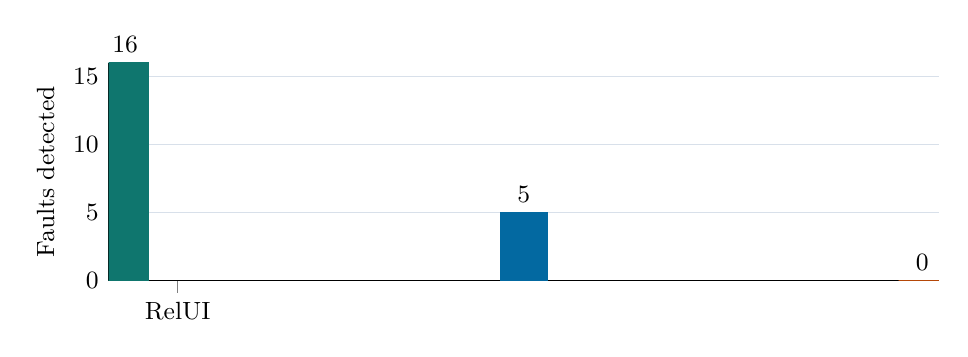
\begin{tikzpicture}
    \begin{axis}[
      ybar,
      ymin=0,
      ymax=16,
      width=\columnwidth,
      height=4.35cm,
      bar width=17pt,
      ylabel={Faults detected},
      symbolic x coords={RelUI,Structural,Visual},
      xtick=data,
      nodes near coords,
      axis lines*=left,
      ymajorgrids=true,
      grid style={draw=reluiLine},
      tick label style={font=\small},
      label style={font=\small},
      every node near coord/.append style={font=\small}
    ]
      \addplot[fill=reluiTeal,draw=reluiTeal] coordinates {(RelUI,16)};
      \addplot[fill=reluiCyan,draw=reluiCyan] coordinates {(Structural,5)};
      \addplot[fill=reluiAmber,draw=reluiAmber] coordinates {(Visual,0)};
    \end{axis}
  \end{tikzpicture}
  \caption{Fault detection comparison. \RelUI detects all 16 injected faults; structural and visual baselines detect 5 and 0.}
  \Description{Bar chart comparing RelUI, structural baseline, and visual baseline.}
  \label{fig:detection-bars}
\end{figure}

\subsubsection{RQ2: Baseline Misses}
Figure~\ref{fig:detection-bars} shows the headline comparison. Structural checking detects five faults that change visible control signatures: one Auth bypass, two Checkout validation failures, and two Transfer validation failures. It misses logout retention, role escalation, payment bypass, cancel/reset persistence, stale quick-save paths, and path-equivalence faults because those failures are semantically wrong but structurally ordinary. The visual baseline detects none under the configured threshold because most faulty pages are intentionally plausible.

\begin{table*}[t]
  \centering
  \caption{Fault coverage matrix. Structural and visual columns show whether the lightweight baselines detected the same faulty variant.}
  \label{tab:fault-matrix}
  \scriptsize
  \begin{tabular}{lllll}
    \toprule
    Fault & Workflow defect & RelUI oracle family & Structural & Visual \\
    \midrule
    F-AUTH-1 & Dashboard bypasses authentication & auth-precondition & \yes & \no \\
    F-AUTH-2 & Logout retains protected access & action-forbidden-state & \no & \no \\
    F-AUTH-3 & User role reaches admin console & auth-precondition & \no & \no \\
    F-AUTH-4 & Invalid login reaches dashboard & validation-blocking & \no & \no \\
    F-CHECKOUT-1 & Invalid contact advances to payment & validation-blocking & \yes & \no \\
    F-CHECKOUT-2 & Express review bypasses payment & action-forbidden-state & \no & \no \\
    F-CHECKOUT-3 & Negative quantity advances checkout & validation-blocking & \yes & \no \\
    F-CHECKOUT-4 & Back path loses contact details & path-equivalence & \no & \no \\
    F-SETTINGS-1 & Quick profile save writes stale state & path-equivalence & \no & \no \\
    F-SETTINGS-2 & Cancel persists edited display name & action-forbidden-state & \no & \no \\
    F-SETTINGS-3 & Reset leaves edited display name & action-forbidden-state & \no & \no \\
    F-SETTINGS-4 & Quick notification save discards state & path-equivalence & \no & \no \\
    F-TRANSFER-1 & Invalid amount advances to recipient & validation-blocking & \yes & \no \\
    F-TRANSFER-2 & Invalid recipient advances to review & validation-blocking & \yes & \no \\
    F-TRANSFER-3 & Receipt reachable without confirm action & auth-precondition & \no & \no \\
    F-TRANSFER-4 & Back/edit path loses transfer amount & path-equivalence & \no & \no \\
    \bottomrule
  \end{tabular}
\end{table*}

\begin{figure}[t]
  \centering
  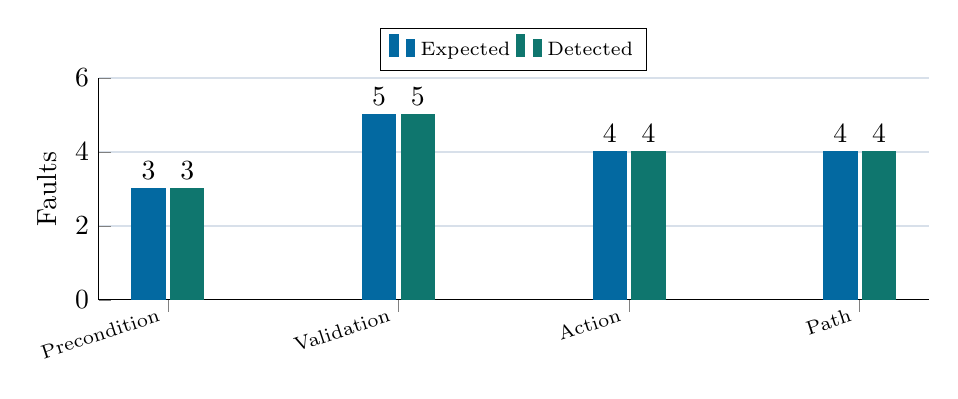
\begin{tikzpicture}
    \begin{axis}[
      ybar,
      ymin=0,
      ymax=6,
      width=\columnwidth,
      height=4.4cm,
      bar width=12pt,
      ylabel={Faults},
      symbolic x coords={Precondition,Validation,Action,Path},
      xtick=data,
      x tick label style={rotate=18,anchor=east,font=\scriptsize},
      legend style={at={(0.5,1.03)},anchor=south,legend columns=2,font=\scriptsize},
      nodes near coords,
      axis lines*=left,
      ymajorgrids=true,
      grid style={draw=reluiLine}
    ]
      \addplot[fill=reluiCyan,draw=reluiCyan] coordinates {(Precondition,3) (Validation,5) (Action,4) (Path,4)};
      \addplot[fill=reluiTeal,draw=reluiTeal] coordinates {(Precondition,3) (Validation,5) (Action,4) (Path,4)};
      \legend{Expected,Detected}
    \end{axis}
  \end{tikzpicture}
  \caption{Invariant-family contribution. Each configured oracle family detects all faults assigned to it.}
  \Description{Grouped bar chart showing expected and detected faults by invariant family.}
  \label{fig:oracle-family}
\end{figure}

\subsubsection{RQ3: Exploration Cost}
Figure~\ref{fig:runtime-model} groups runtime and model size by workflow. Checkout is slowest at 91.77 seconds because it has the deepest workflow and largest transition set. Transfer adds 122 traces and 127 transitions in 72.10 seconds, showing that the added benchmark increases evaluation breadth without dominating total cost. Settings is smallest because most traces are short profile or notification actions.

\begin{figure*}[t]
  \centering
  \begin{subfigure}[t]{0.47\textwidth}
    \centering
    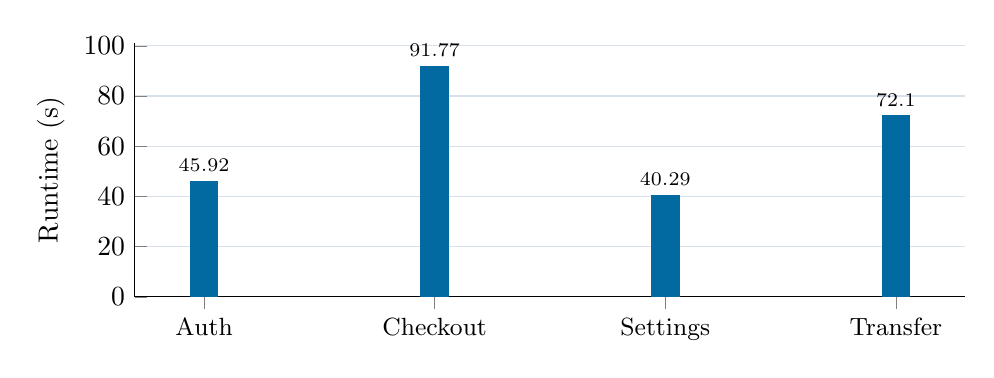
\begin{tikzpicture}
      \begin{axis}[
        ybar,
        width=\linewidth,
        height=4.8cm,
        ymin=0,
        ylabel={Runtime (s)},
        symbolic x coords={Auth,Checkout,Settings,Transfer},
        xtick=data,
        x tick label style={font=\small},
        nodes near coords,
        every node near coord/.append style={font=\scriptsize},
        axis lines*=left,
        ymajorgrids=true,
        grid style={draw=reluiLine}
      ]
        \addplot[fill=reluiCyan,draw=reluiCyan] coordinates {(Auth,45.92) (Checkout,91.77) (Settings,40.29) (Transfer,72.10)};
      \end{axis}
    \end{tikzpicture}
    \caption{Runtime by workflow.}
  \end{subfigure}
  \hfill
  \begin{subfigure}[t]{0.49\textwidth}
    \centering
    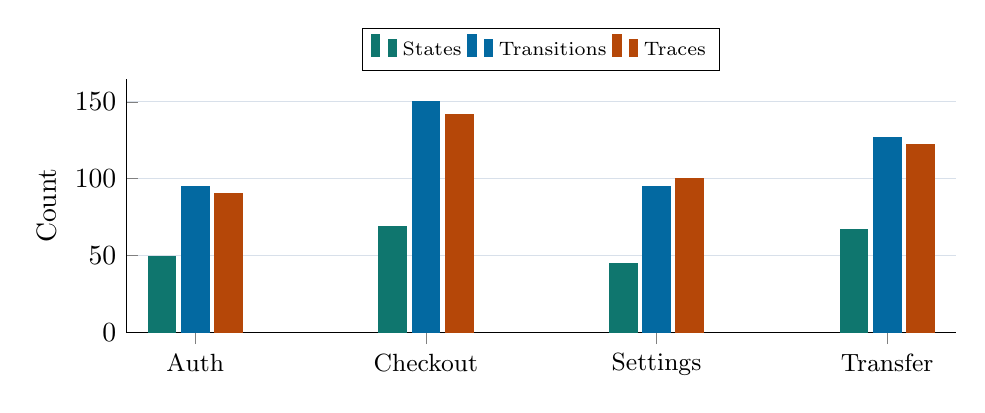
\begin{tikzpicture}
      \begin{axis}[
        ybar,
        width=\linewidth,
        height=4.8cm,
        ymin=0,
        ylabel={Count},
        symbolic x coords={Auth,Checkout,Settings,Transfer},
        xtick=data,
        legend style={at={(0.5,1.03)},anchor=south,legend columns=3,font=\scriptsize},
        axis lines*=left,
        ymajorgrids=true,
        grid style={draw=reluiLine},
        x tick label style={font=\small}
      ]
        \addplot[fill=reluiTeal,draw=reluiTeal] coordinates {(Auth,49) (Checkout,69) (Settings,45) (Transfer,67)};
        \addplot[fill=reluiCyan,draw=reluiCyan] coordinates {(Auth,95) (Checkout,150) (Settings,95) (Transfer,127)};
        \addplot[fill=reluiAmber,draw=reluiAmber] coordinates {(Auth,90) (Checkout,142) (Settings,100) (Transfer,122)};
        \legend{States,Transitions,Traces}
      \end{axis}
    \end{tikzpicture}
    \caption{Inferred model size and traces.}
  \end{subfigure}
  \caption{Runtime and model size after adding Transfer. The cost tracks workflow depth and branching more than the number of variants alone.}
  \Description{Two charts: runtime by app and grouped bars for states, transitions, and traces.}
  \label{fig:runtime-model}
\end{figure*}

\subsubsection{Representative Counterexample}
Figure~\ref{fig:transfer-counterexample} shows the new Transfer path-equivalence fault. A normal transfer receipt preserves \texttt{\$125}; the back/edit path reaches the same receipt state class after confirmation but loses the amount. The page remains visually plausible, which explains why local visual comparison is weak here.

\begin{figure*}[t]
  \centering
  \begin{subfigure}[t]{0.48\textwidth}
    \centering
    \artifactimage[width=\linewidth]{artifacts/subjects/transfer-back-loses-transfer/screenshots/s_8cdb85b8f356.png}
    \caption{Normal path: confirmed receipt keeps the amount.}
  \end{subfigure}
  \hfill
  \begin{subfigure}[t]{0.48\textwidth}
    \centering
    \artifactimage[width=\linewidth]{artifacts/subjects/transfer-back-loses-transfer/screenshots/s_29cb5e1f4e4a.png}
    \caption{Back/edit path: receipt loses the amount.}
  \end{subfigure}
  \caption{Transfer counterexample for F-TRANSFER-4. The two traces both end after \texttt{confirm-transfer}, but endpoint fingerprints differ: one receipt reports \texttt{Amount: \$125}, while the other reports \texttt{Amount: missing}.}
  \Description{Two transfer receipt screenshots showing preserved amount versus missing amount.}
  \label{fig:transfer-counterexample}
\end{figure*}

\FloatBarrier
\section{Related Work}
\textbf{Model-based testing.} Model-based testing derives tests from behavioral models \citep{utting2012taxonomy}. \RelUI also uses a transition model, but infers it from browser traces and uses it mainly for relational oracle checking rather than for exhaustive model-derived generation.

\textbf{Web state crawling and invariants.} Crawljax explores Ajax applications and infers state-flow graphs \citep{mesbah2012crawling}. Invariant-based Web testing checks discovered states against state and DOM constraints \citep{mesbah2012invariant}. \RelUI builds on these ideas but checks relationships between traces: required actions before protected endpoints, invalid profiles before forbidden states, and equivalent paths to the same task endpoint.

\textbf{GUI testing frameworks.} GUITAR provides an extensible GUI testing framework across workflows and platforms \citep{nguyen2013guitar}. \RelUI is narrower and Web-focused, but produces compact Playwright replay evidence around relational workflow defects.

\textbf{Browser automation and LVLM GUI testing.} Playwright supplies reliable browser automation and screenshots \citep{playwright}. LVLM-based tools such as VETL use visual understanding for GUI exploration and input generation \citep{wang2024vetl}. \RelUI is complementary: its oracle is explicit and auditable rather than learned.

\section{Threats to Validity}
\textbf{Internal validity.} The faults are controlled injections, and each expected fault is mapped to an invariant in the configuration. This improves auditability but means results depend on the correctness of those mappings. Clean variants reduce false-positive risk, but they do not prove the invariants are complete.

\textbf{External validity.} The four workflows are realistic surrogates, not production systems. They cover authentication, checkout, settings, and transfer behavior, but not all asynchronous, third-party, or highly dynamic UI patterns.

\textbf{Construct validity.} The structural and visual baselines are lightweight diagnostic baselines. Their role is to show that local structure and appearance miss relational defects, not to replace a full comparison with mature commercial suites.

\textbf{Reliability.} \RelUI resets browser storage before traces and uses deterministic input profiles. Remaining nondeterminism can come from browser timing and screenshots. The artifact preserves graphs, traces, screenshots, CSV files, and HTML evidence to support reruns and manual inspection.

\section{Conclusion}
\RelUI shows that Web UI correctness often depends on relationships across actions and paths. The final artifact expands the evaluation to four workflows, 20 variants, and 16 injected faults; it detects all faults with zero clean false positives while local structural and visual baselines detect only 5 and 0. The results support the core claim: workflow-level UI testing needs explicit relational oracles, not only page-local checks.

\bibliographystyle{ACM-Reference-Format}
\IfFileExists{references.bib}{\bibliography{references}}{\bibliography{pdf/references}}

\end{document}
